\section{Gender}
\label{sec:warmup3}

    In this preliminary practice activity, we were given chest X-ray images of patients using which we have to either train or fine-tune a model to determine the gender of patients.

\subsection{Dataset}
    We were given three datasets for classifying gender of the patients; grayscale, RGB, and index. Out of these, I have used Gender01\_RGB for the experiments. The provided dataset 154 training samples of patient X-Rays and an additional 93 samples for testing trained model.  The images in this dataset were color image with shape $256$x$256$. Each training samples have either label "male", or "female". Due to the absence of a dedicated validation set in this dataset too, I have randomly partitioned the training samples into training and validation sets in 9:1 ratio.

\subsection{Training}

    In this task, we are dealing with two labels: male and female. Therefore, we constructed a model with a graph described in \cref{fig:gender_model}. A log-softmax layer is employed to obtain probabilities for each class. The model is trained using the categorical cross-entropy loss function with Adam optimizer having a learning rate of $0.003$. We utilize the torch.nn.NLLLoss function, which is commonly used for classification problems, as our loss function. Additionally, early stopping with a patience of 3 epochs is implemented to halt the model training if the validation loss continues to increase for 3 consecutive epochs. \Cref{fig:gender-learning-curve} illustrates the learning curve of the training and validation sets.

    \begin{figure}[htbp]
        \centering
        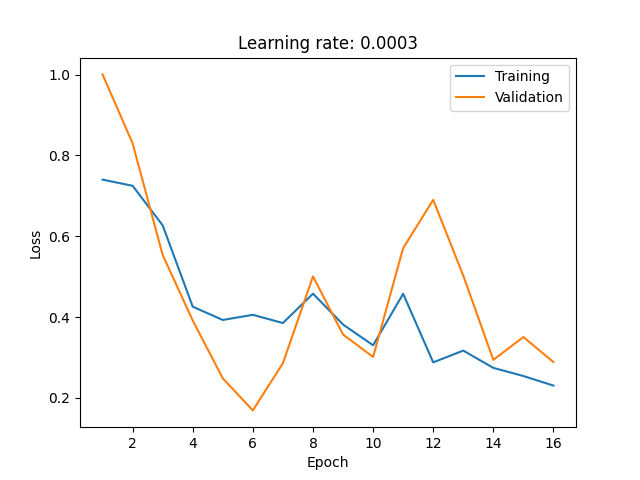
\includegraphics[width=\linewidth]{../outputs/gender/gender1/loss-curve.png}
        \caption{Gender model learning curve on training and validation sets}
        \label{fig:gender-learning-curve}
    \end{figure}

\subsection{Results}

    \begin{figure}[!htbp]
        \centering
        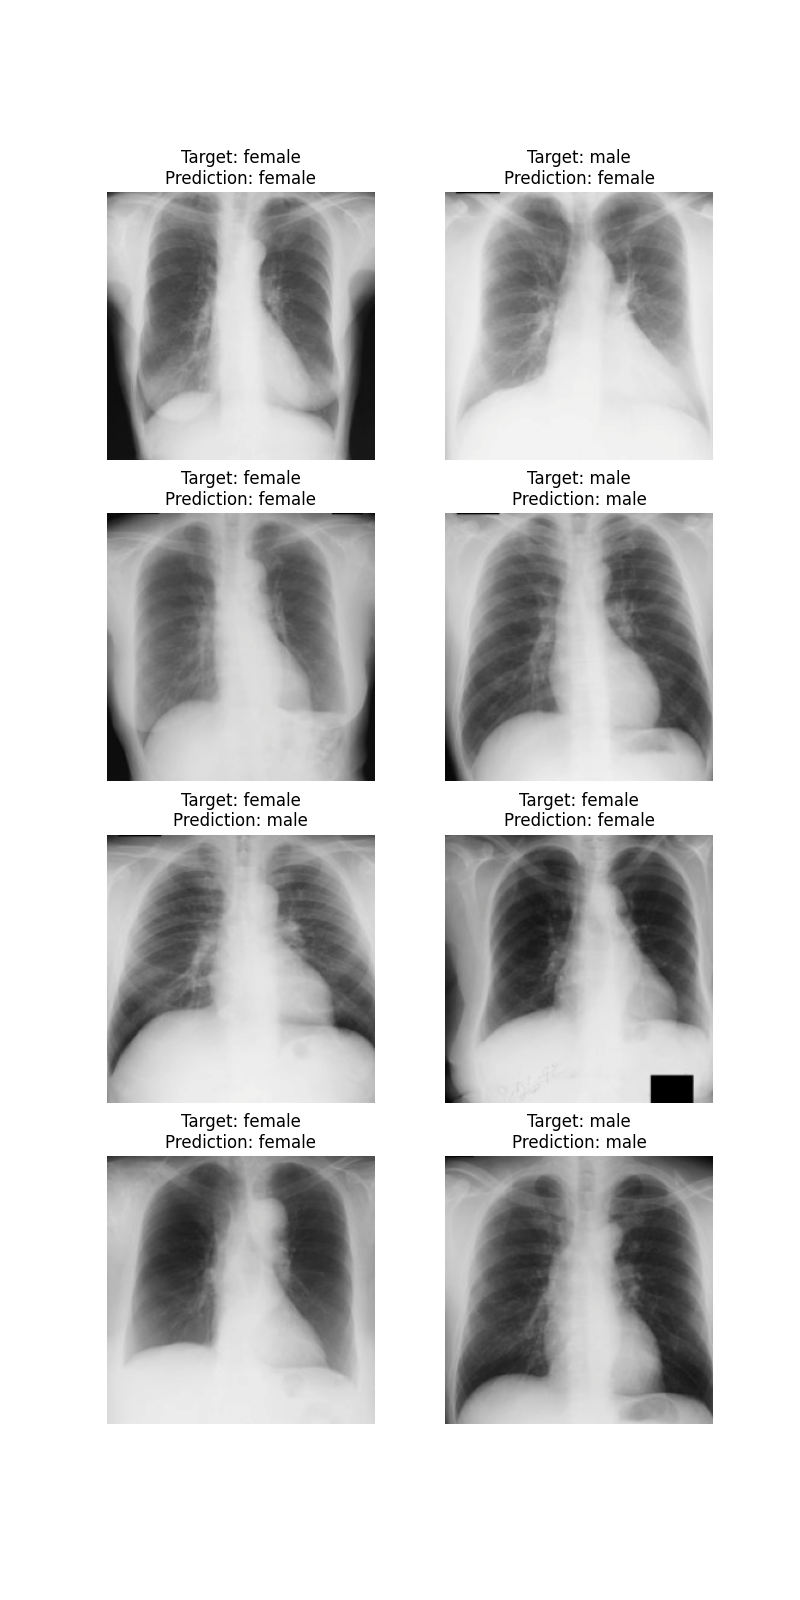
\includegraphics[width=\linewidth]{../outputs/gender/gender1/test-results.png}
        \caption{Gender predictions on few samples of test data}
        \label{fig:gender-results}
    \end{figure} 

    After fine-tuning the model, it was evaluated on the provided test samples on which it achieved an accuracy of $90.32\%$, and AUC of $90.34$. \Cref{fig:gender-results} showcases some of the test samples along with their model predictions and target classes.
